%!TEX root = ../main.tex
\section{Evaluation}
\label{sec: mercury_evaluation}
We now present the evaluation of our \textit{Assisted I/O library} and \textit{Advice Manager} prototypes with a real world application used by physicists at the data processing center of the University of Mainz (ZDV). Our testbed is composed by %two separate systems: 
a test cluster of seven nodes, mainly intended to evaluate the proposed Linux kernel modification with the Lustre file system. %, and the Mogon cluster, currently the production system at the ZDV. 
We start with a concise description of the %two 
system as well as a detailed analysis of the target application's I/O pattern, and then present the results of our experiments. 

We evaluate the performance of our framework using two metrics, the execution time of the test application and the number of reads completed by every target file system. %To simulate a heavily loaded cluster we use a background process that runs on an set of nodes independent from the node running the target application. Additionally, we also measure the overhead introduced by our prototype. 

\subsection{Test Cluster}
\label{subsec: test_cluster}
%Markus description
As already mentioned, this small cluster is aimed mainly to test our modified kernel with Lustre. The reason is that it was not possible to disrupt the production cluster, affecting hundreds of users, by re-installing the operating system kernel. In order to make realistic comparisons between Lustre and GPFS, the test cluster also has a GPFS file system on comparable hardware. Both filesystems have a single disk server each, one Dell R710 acts as GPFS network shared disk (NSD) server and another as Lustre object storage server (OSS). The R710 are equipped with two quadcore E5620 @ 2.4 GHz and 24 GB main memory. For storage, both disk servers share a MD3200 array with 2 controllers and 4 MD1200 expansion shelves for a total of 60 2 TB drives. The Storage is formatted in 4 15 dynamic disk pools. This is the LSI/Netapp type of declustered RAID, which distributes the 8+2 RAID6 stripes evenly over all 15 disks for better rebuild performance. The disk block size is set to 128 KiB, which results in a RAID stripe size of 1MiB. The four disk pools are then split on the Array into LUNs, one of the LUNs from each disk pool is then used for GPFS and another one from each pool is used for Lustre. This results in comparable resources for both filesystems and tests do not interfere with each other, as long as only one filesystem is tested at a time. While the GPFS filesystem embeds the metadata with the data, Lustre needs a separate Metadata Server (MDS). This is hosted by a SuperMicro server equipped with one quadcore Xeon E3-1230 @3.3 GHz and 16 GB of main memory, as metadata target (MDT) it uses a 120 GB SSD Intel 520. Four other machines of the same type, equipped with an eight core E3-1230 @3.3 GHz processor and 16 GB of main memory, work as compute nodes and file system clients. All machines, servers and clients, are equipped with Intel X520DA 10 Gigabit adapters and connected to a SuperMicro SSE-X24S 24 ports 10 Gigabit switch. Both, the GPFS and Lustre file systems are formatted with a block size of 4 MB.

\subsection{Real World Application}
\label{subsec: application}
Our target real world application is written using `ROOT', an object-oriented framework widely adopted in the experimental high energy physics community to build software for data analysis. The application analyzes data read from an input file in the `ROOT' format (structured file format). 

\begin{figure*}[!htb]
  \centering
  \begin{subfigure}[t]{0.48\textwidth}
    \centering
    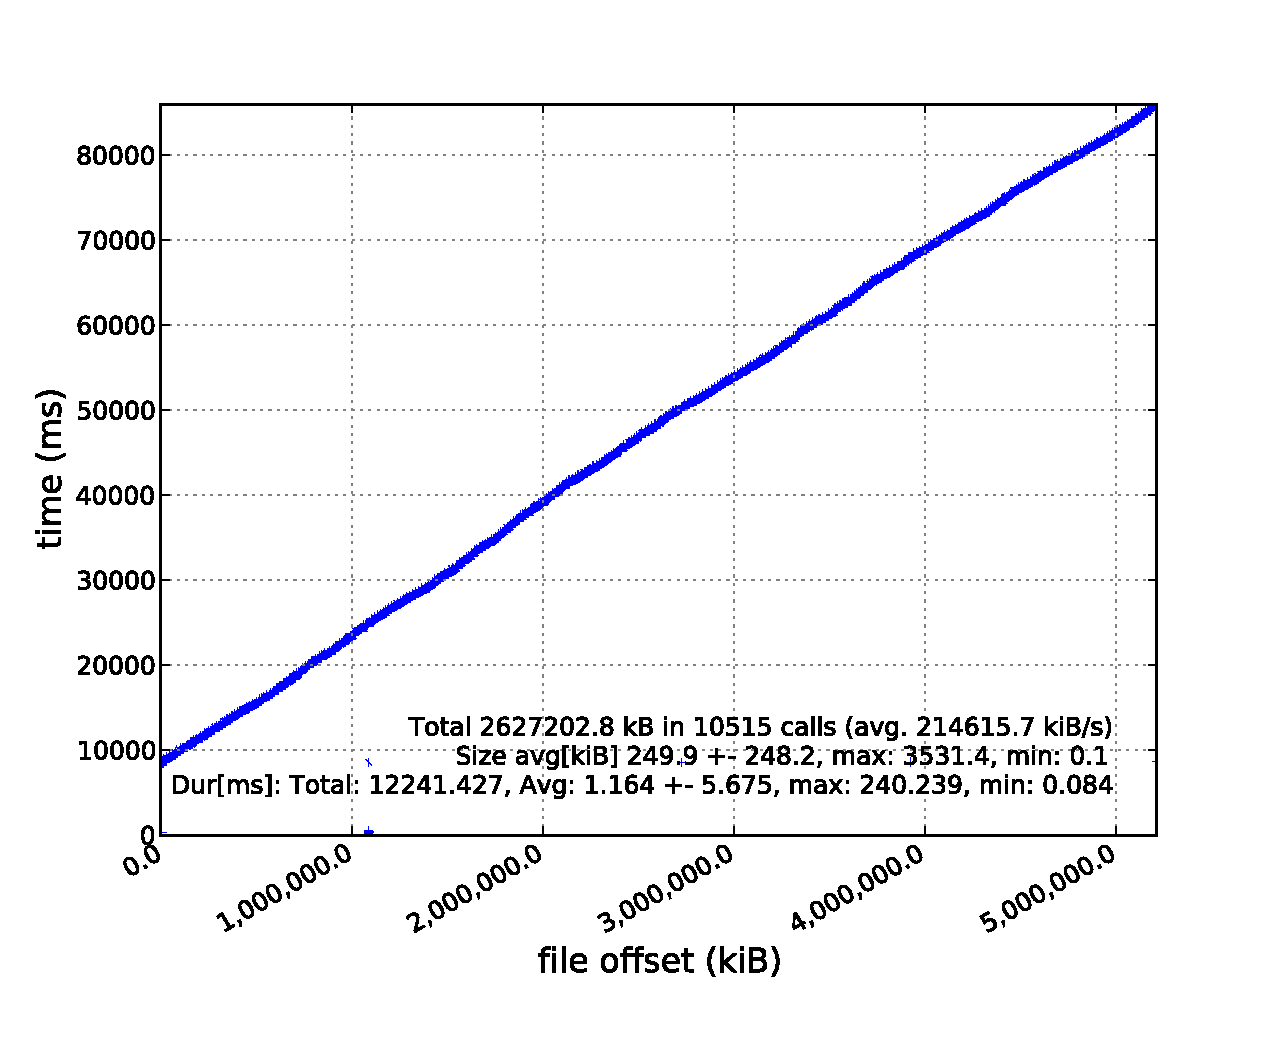
\includegraphics[width=\textwidth]{chapters/chapter2/figures/iopat_profile}
    \caption{\textit{}}
    \label{figure: iopat_profile}
  \end{subfigure}
  \begin{subfigure}[t]{0.48\textwidth}
    \centering
    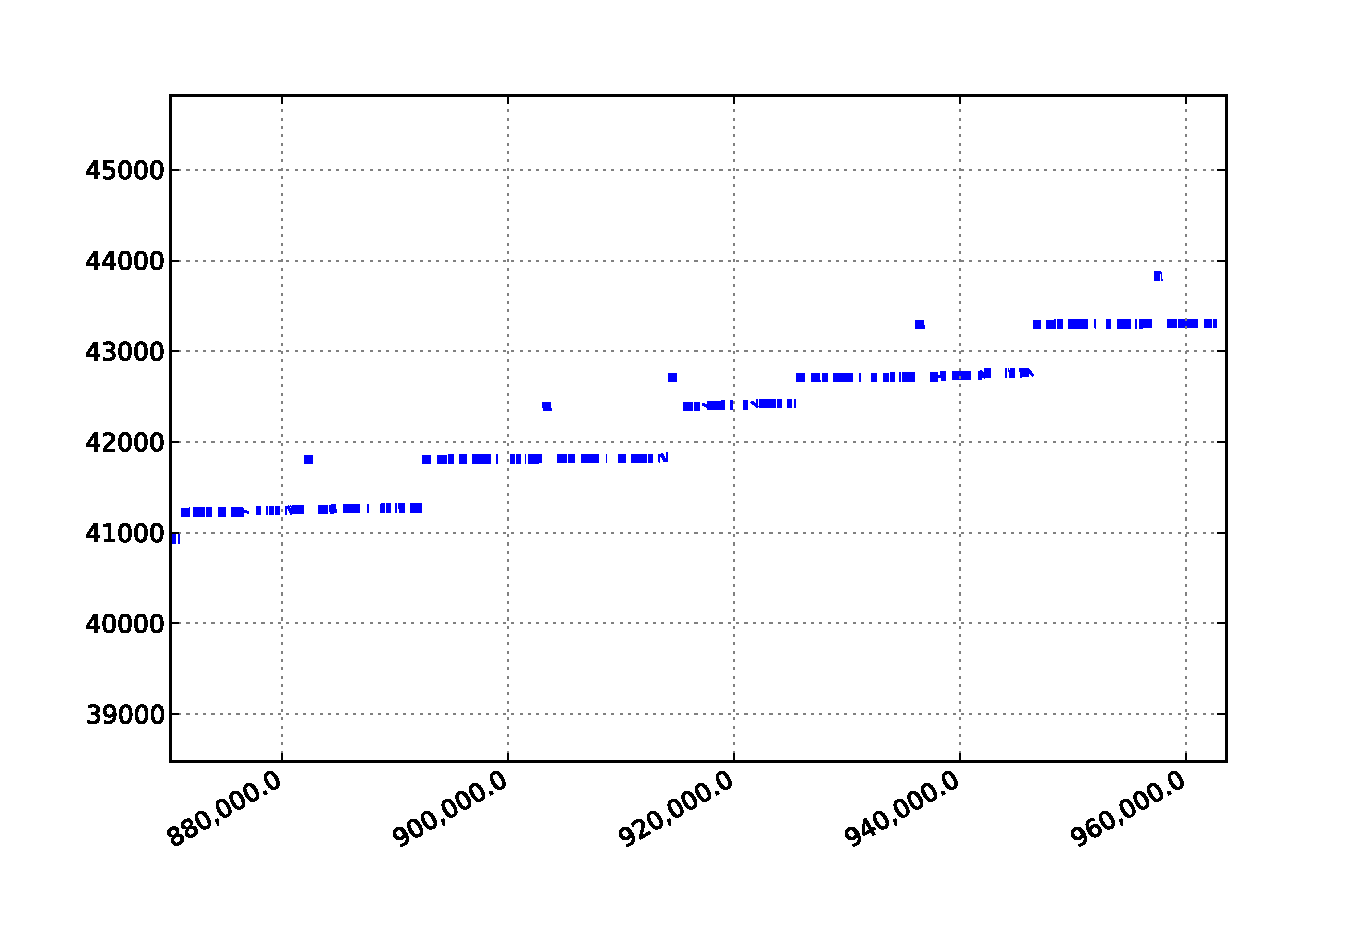
\includegraphics[width=\textwidth]{chapters/chapter2/figures/00050_zoom}
    \caption{\textit{}}
    \label{figure: iopat_zoom}
  \end{subfigure}
  \caption{I/O read profile of the target application under analysis (\ref{figure: iopat_profile}), extracted from the the GPFS file system in the test cluster, and zoomed window (\ref{figure: iopat_zoom}) showing the actual pattern details.}
  \label{figure: iopattern_with_statistics}
\end{figure*}

First of all we characterized the application's I/O pattern for a target file using traces and statistics extracted through several tools such as \textit{strace}, \textit{ioapps}~\cite{ioapps} and GPFS's \textit{mmpmon}~\cite{mmpmon} monitoring tool. Figure~\ref{figure: iopattern_with_statistics} shows the I/O pattern along with some additional statistics. As it can be seen, in this specific case (5 GB file), the application issues a total of 10515 \texttt{read()} system calls to read about 2.6 GB of total data. The average request size is 250 kiB and the time spent waiting for I/O is 12 seconds, when running on the test cluster. 

At a first glance the general I/O behaviour of the application looks linear, most of the accesses to the file follow an increasing offset. Nevertheless, adjacent reads are separated by gaps (a strided read pattern). In a few cases this gap becomes negative, meaning that the application is moving backwards in the file to read some data previously left behind (as reported in Figure~\ref{figure: iopat_zoom}). %(Figure~\ref{figure: 00050_zoom}). 

After a detailed I/O pattern analysis we could divide the target file into contiguous non overlapping ranges. Within these ranges reads happen to have increasing offset. Even though the general I/O pattern of the application for different files looks similar\footnote{Due to space limits we do not report the comparison between different files.}, the size of the non overlapping ranges may change significantly. This general behaviour can be modelled using a configuration file in which a `WillNeed' hint covers the whole file from beginning to end (i.e. `Offset' and `Length' equal to 0). The backwards seeks can be accounted for using the `CacheSize' parameter to keep previously accessed blocks in cache. In this way we effectively emulate a sliding window that tracks the application's I/O behaviour. This would not be possible by just using a, e.g., \texttt{POSIX\_FADV\_WILLNEED} advice on the whole file before starting the application like shown by Figure~\ref{figure: fadvise_comparison}. The reason is that if the file size is equal or smaller than the cache size, we would have a large number of valuable pages discarded from the cache to load data that will be accessed at the end of the application. Additionally, if the file size is bigger than the cache size we would have the file system discarding blocks at the beginning of the file as the blocks at the end are preloaded, effectively forcing the application to access these blocks from the I/O servers instead of the cache. With our approach, on the other hand, we keep in the cache only a small, controlled number of blocks (the ones currently accessed), while the older blocks are discarded since no longer needed. 

\begin{figure}[!htb]
  \centering
  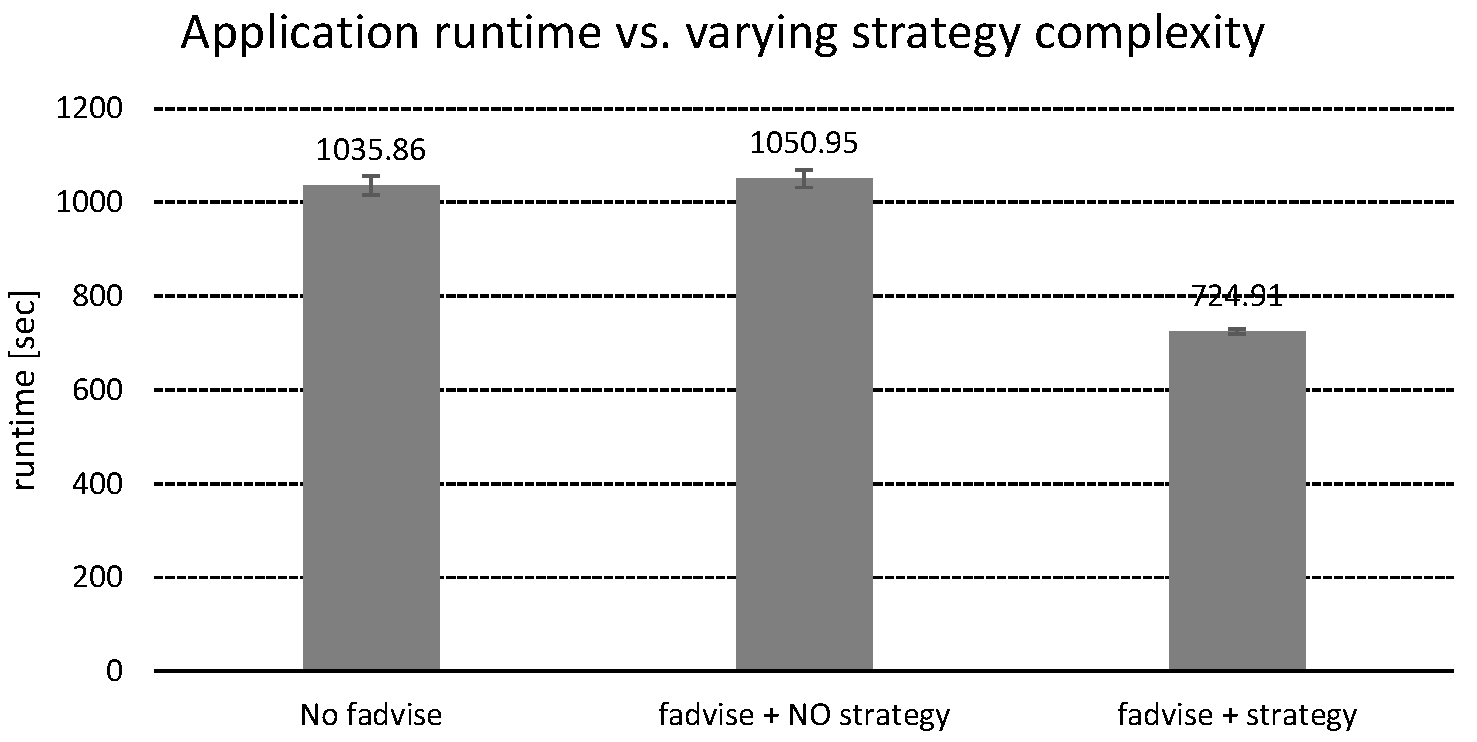
\includegraphics[width=0.8\textwidth]{chapters/chapter2/figures/SC2015/ROOT/separate_plots/test_cluster/test_fadvise_no_border}
  \caption{Comparison between different usage stategies of posix\_fadvise for an input file of 55 GB residing in an ext4 file system. The first bar represents the case in which no advice is used, the second bar represents the case in which a POSIX\_FADV\_WILLNEED is issued for the whole file at the beginning of the application and the third bar represents the case in which POSIX\_FADV\_WILLNEED is issued using MERCURY.}
  \label{figure: fadvise_comparison}
\end{figure} 
 
To assess the impact of our prototype on the application and file systems performance we considered the application execution time and the number of reads accounted for by the respective file systems. We conducted our experiments without file system hints and then with file system hints issued transparently to the application by the \textit{Advice Manager}. Furthermore, we ran each experiment three times and calculated average, minima and maxima for each metric. In order to avoid caching affecting our measurements, extra care was taken to clean all the relevant caches for the different file systems. For ext4 and Lustre this was accomplished by using the command line: $$echo\ 3 > /proc/sys/vm/drop\_caches$$ on the file system clients. Additionally, for Lustre this command was also executed on the OSS to avoid the server side cache to be retained. In the case of GPFS, the file system client's page pool was cleaned using the clean file cache hint in Table~\ref{table: hints_table}, the NSD servers do not cache any data. 

\subsection{Execution Time}
\label{subsec: results}
To measure the performance improvements that our prototype can deliver to the application's runtime we conducted two set of tests. In the first test we varied the size of the input file from 5 to 95 GB. This is mainly aimed to study the behaviour of the `ROOT' application using different input file sizes and how our solution behaves when the file becomes bigger than the available cache space. In the second test we varied the number of `ROOT' instances running simultaneously from 1 to 8. By doing so we study the interaction of multiple processes accessing the file system and how these can benefit from the prefetching hints generated by MERCURY. Figure~\ref{figure: runtime} reports the results for the described experiments. All the tests where performed using a `BlockSize' of 4 MB, a `CacheSize' of 8 blocks, a `ReadAheadSize' of 4 blocks, and a `WillNeed' hint covering the whole file (i.e. with `Offset' and `Length' equal to 0), resulting in each process consuming up to 32 MB of cache space and 512 MB in total for 8 application instances. The `WillNeed' on the whole file causes the \textit{Advisor Thread} to issue up to 4 (`ReadAheadSize') prefetching requests for blocks of 4 MB sequentially, starting from the current accessed block. This has the same effect of data sieving in ROMIO, optimizing the access size and allowing the application to read the requested data randomly from the cache instead of the file system. The produced effect is particularly beneficial in the case of Lustre and ext4, as it can be seen in Figures~\ref{figure: ext4_1} and~\ref{figure: lustre_1}. In these cases we measure reductions in the execution time of up to 50\% circa, with respect to the normal case. For GPFS we can still observe an improvement but this is more contained compared to the other file systems (Figure~\ref{figure: gpfs_1}). The reductions in the execution time measured in GPFS are on average up to 10\%, with respect to the normal case. The reason is that the default prefetching strategy in GPFS works better that traditional read-ahead. In fact, by disabling the prefetching in GPFS we observed reductions in the execution time comparable to the other file systems (not reported here).
\begin{figure*}[!htb]
  \centering
  \begin{subfigure}[t]{0.32\textwidth}
    \centering
    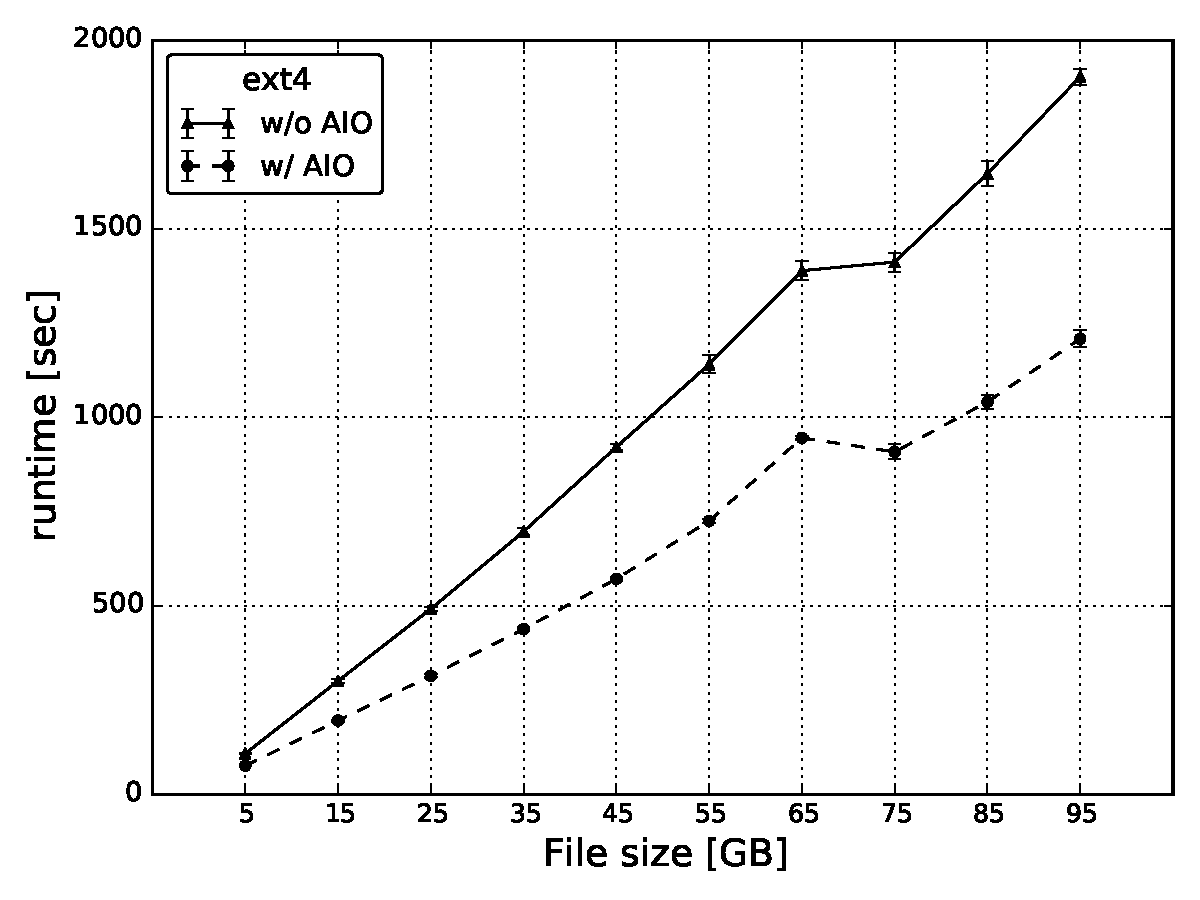
\includegraphics[width=\textwidth]{chapters/chapter2/figures/SC2015/ROOT/separate_plots/test_cluster/ext4/runtime}
    \caption{\textit{}}
    \label{figure: ext4_1}
  \end{subfigure}
  \begin{subfigure}[t]{0.32\textwidth}
    \centering
    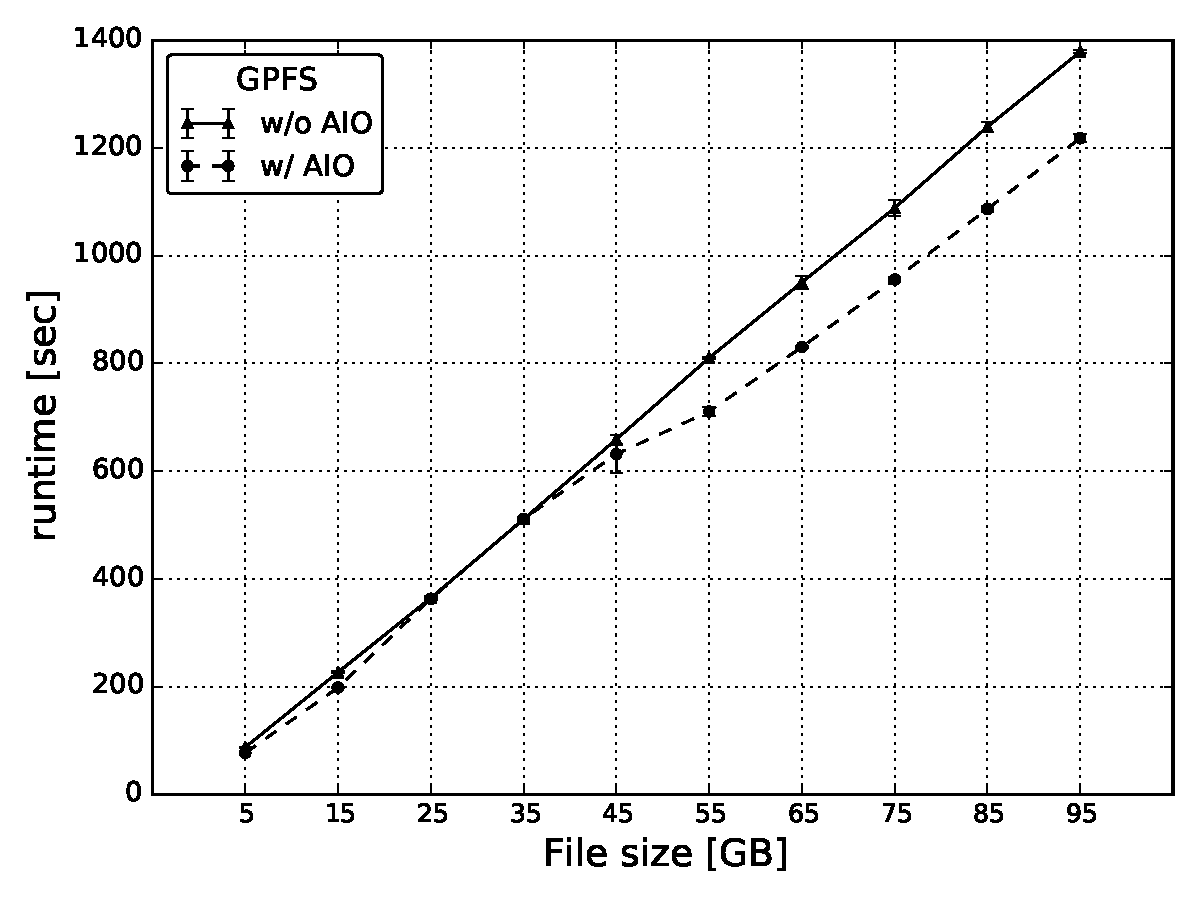
\includegraphics[width=\textwidth]{chapters/chapter2/figures/SC2015/ROOT/separate_plots/test_cluster/gpfs/runtime}
    \caption{\textit{}}
    \label{figure: gpfs_1}
  \end{subfigure}
  \begin{subfigure}[t]{0.32\textwidth}
    \centering
    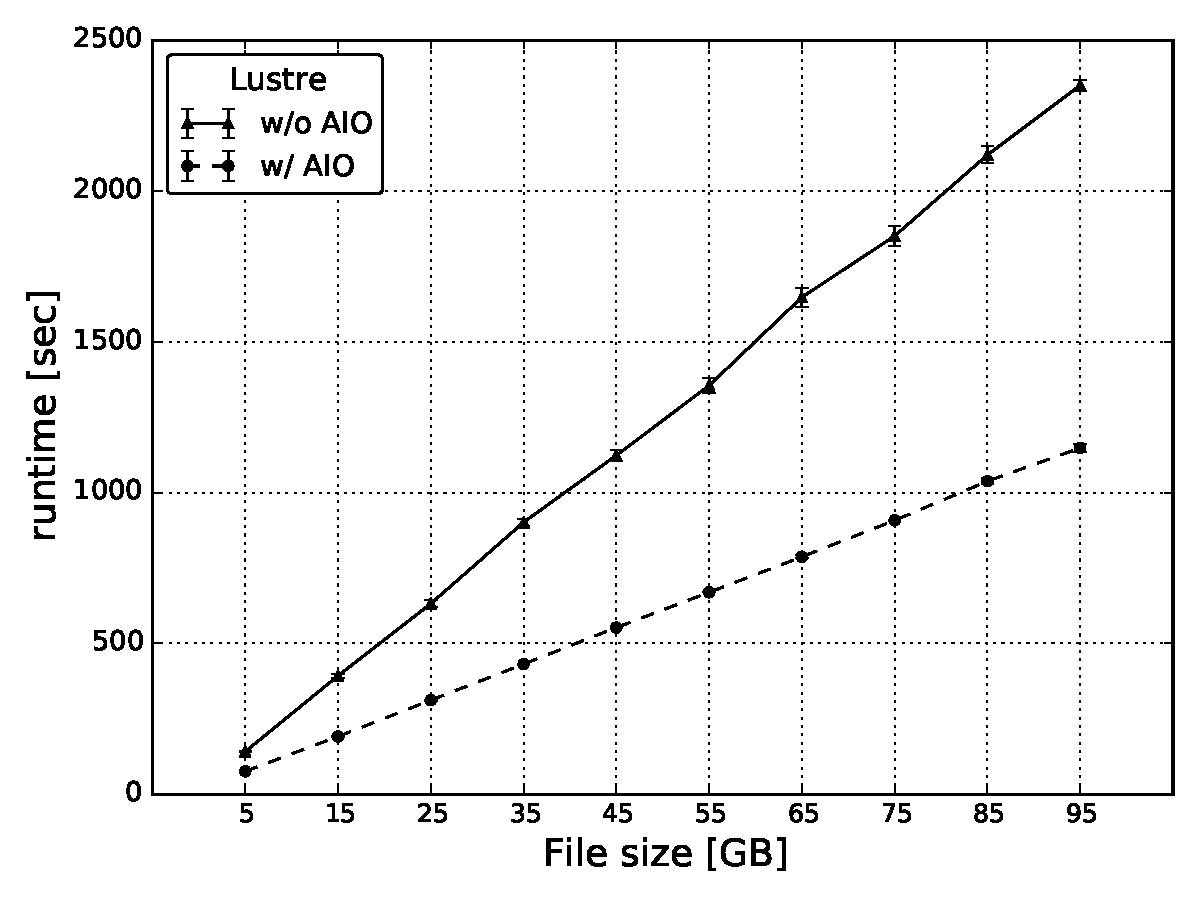
\includegraphics[width=\textwidth]{chapters/chapter2/figures/SC2015/ROOT/separate_plots/test_cluster/Lustre/runtime}
    \caption{\textit{}}
    \label{figure: lustre_1}
  \end{subfigure}
  \begin{subfigure}[b]{0.32\textwidth}
    \centering
    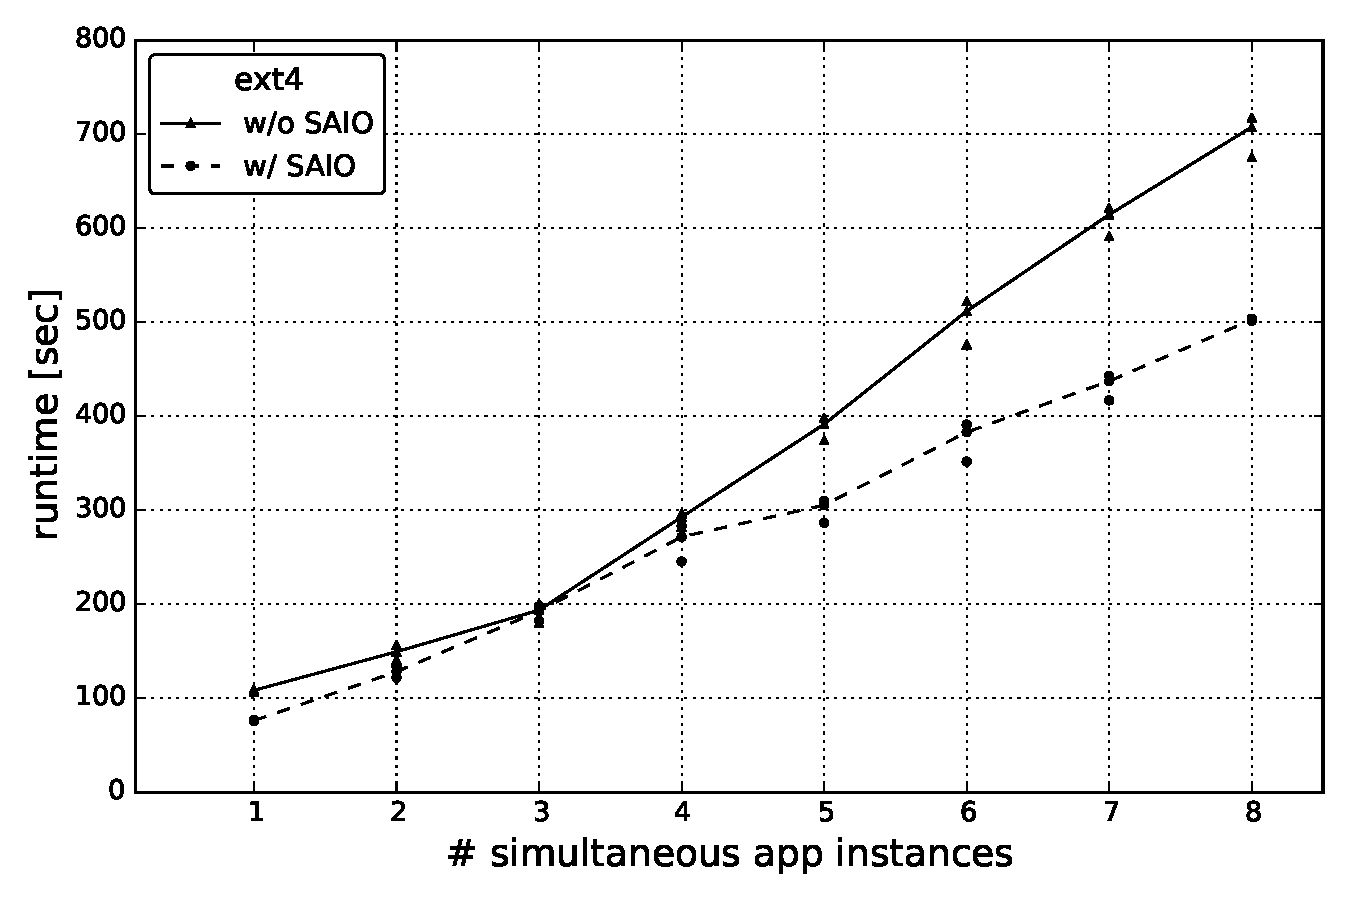
\includegraphics[width=\textwidth]{chapters/chapter2/figures/SC2015/ROOT/cluster/multiple_instances/simult_instance_ext4_test_cluster}
    \caption{\textit{}}
    \label{figure: ext4_2}
  \end{subfigure}
  \begin{subfigure}[b]{0.32\textwidth}
    \centering
    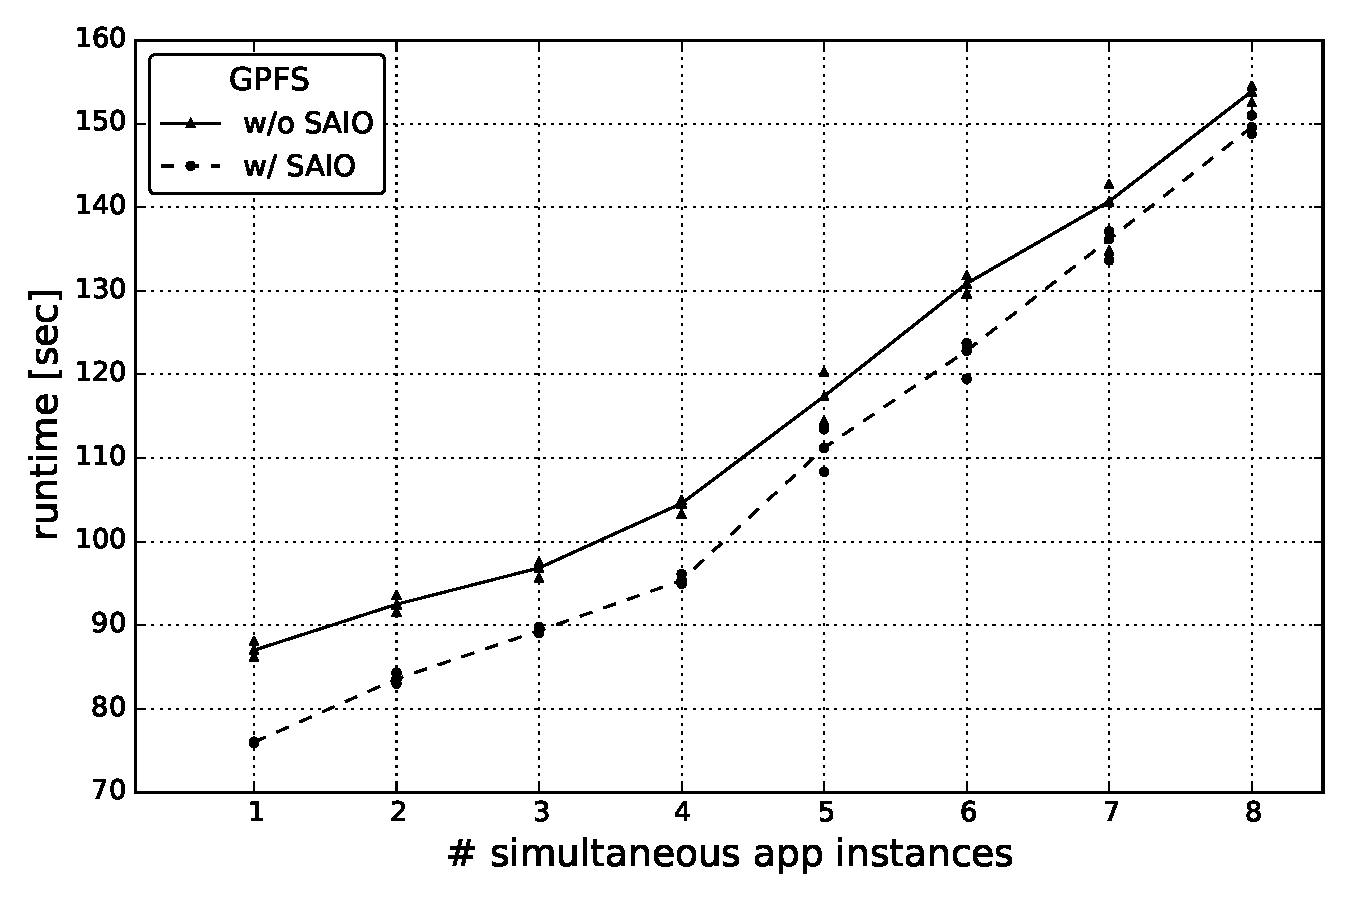
\includegraphics[width=\textwidth]{chapters/chapter2/figures/SC2015/ROOT/cluster/multiple_instances/simult_instance_gpfs_test_cluster}
    \caption{\textit{}}
    \label{figure: gpfs_2}
  \end{subfigure}
  \begin{subfigure}[b]{0.32\textwidth}
    \centering
    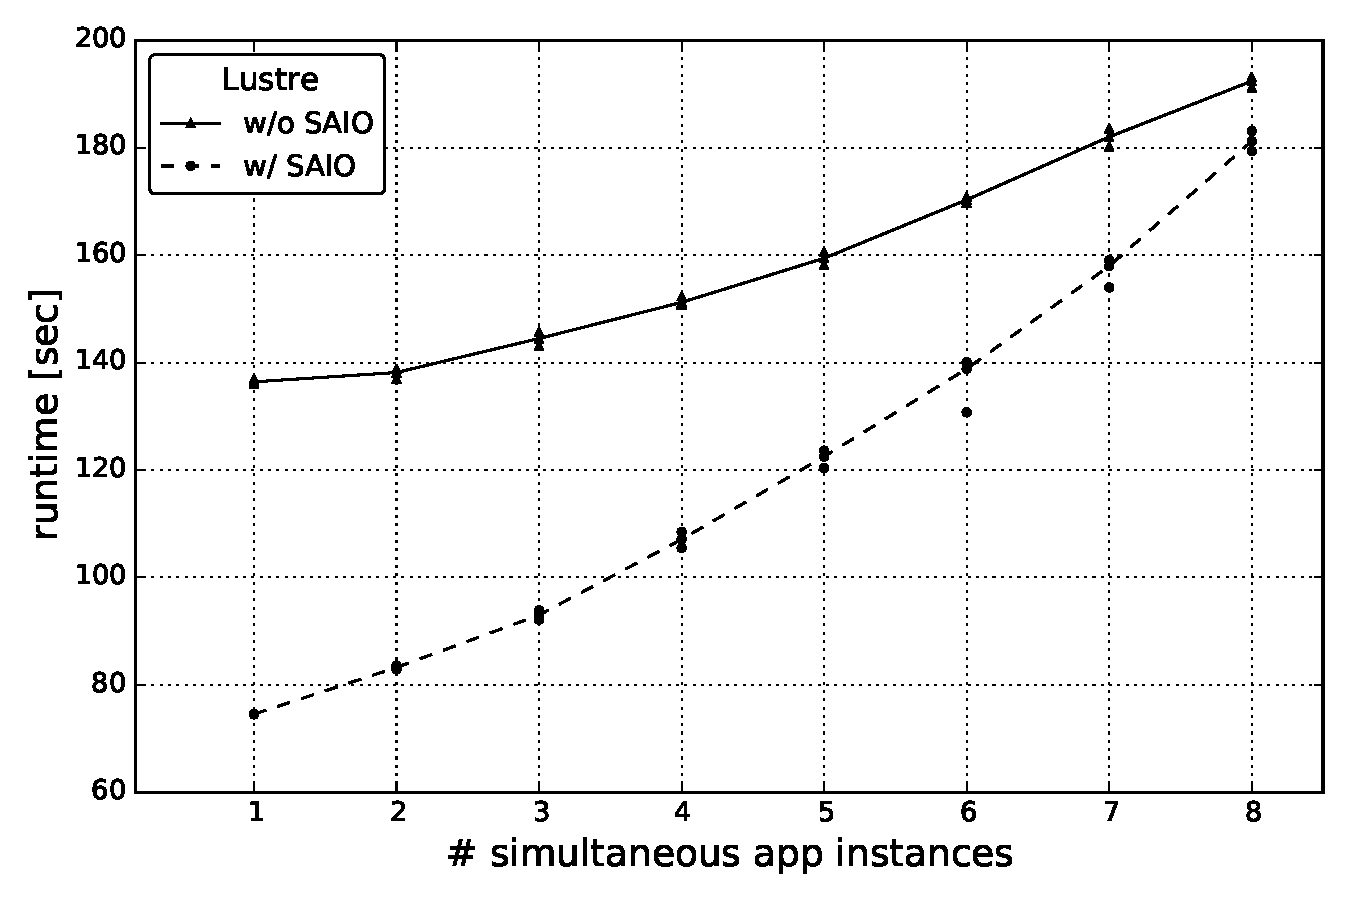
\includegraphics[width=\textwidth]{chapters/chapter2/figures/SC2015/ROOT/cluster/multiple_instances/multiple_simult_procs_Lustre_testcluster}
    \caption{\textit{}}
    \label{figure: lustre_2}
  \end{subfigure}
  \caption{Running time of the ROOT application for the three file system under study using different input file sizes (\ref{figure: ext4_1},~\ref{figure: gpfs_1} and~\ref{figure: lustre_1}) and different number of instances accessing a file of 5 GB (\ref{figure: ext4_2},~\ref{figure: gpfs_2} and~\ref{figure: lustre_2}).}
  \label{figure: runtime}
\end{figure*}
\begin{figure*}[!htb]
  \centering
  \begin{subfigure}[t]{0.32\textwidth}
    \centering
    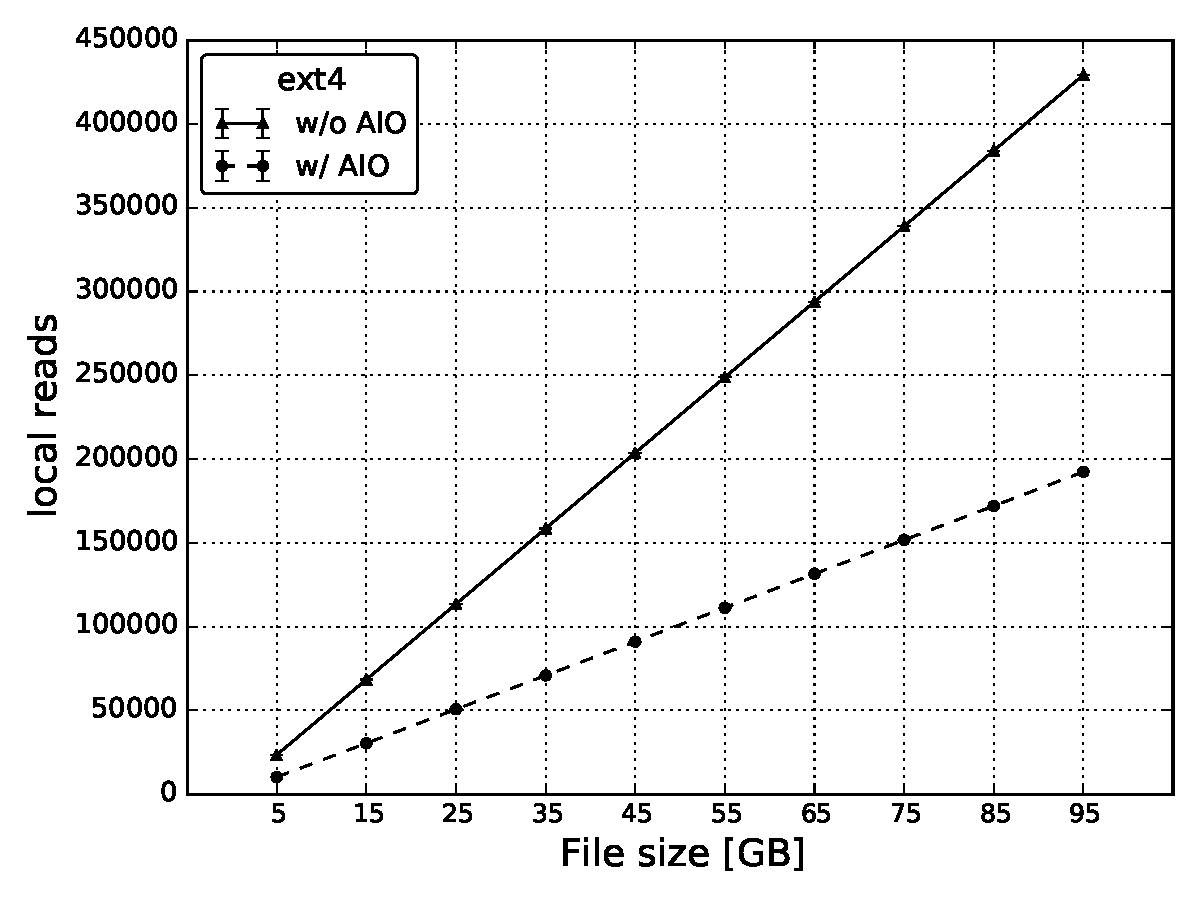
\includegraphics[width=\textwidth]{chapters/chapter2/figures/SC2015/ROOT/separate_plots/test_cluster/ext4/reads}
    \caption{\textit{}}
    \label{figure: ext4_3}
  \end{subfigure}
  \begin{subfigure}[t]{0.32\textwidth}
    \centering
    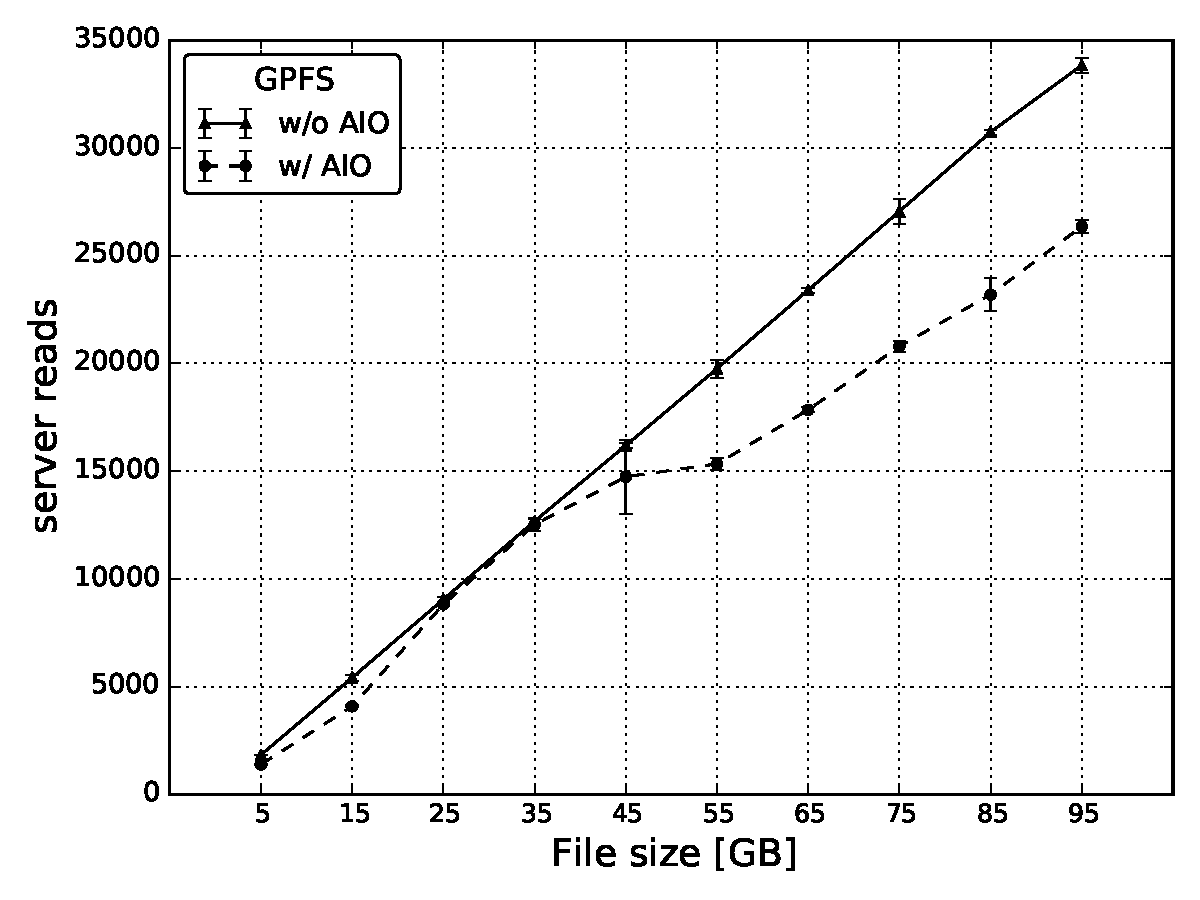
\includegraphics[width=\textwidth]{chapters/chapter2/figures/SC2015/ROOT/separate_plots/test_cluster/gpfs/server_reads}
    \caption{\textit{}}
    \label{figure: gpfs_3}
  \end{subfigure}
  \begin{subfigure}[t]{0.32\textwidth}
    \centering
    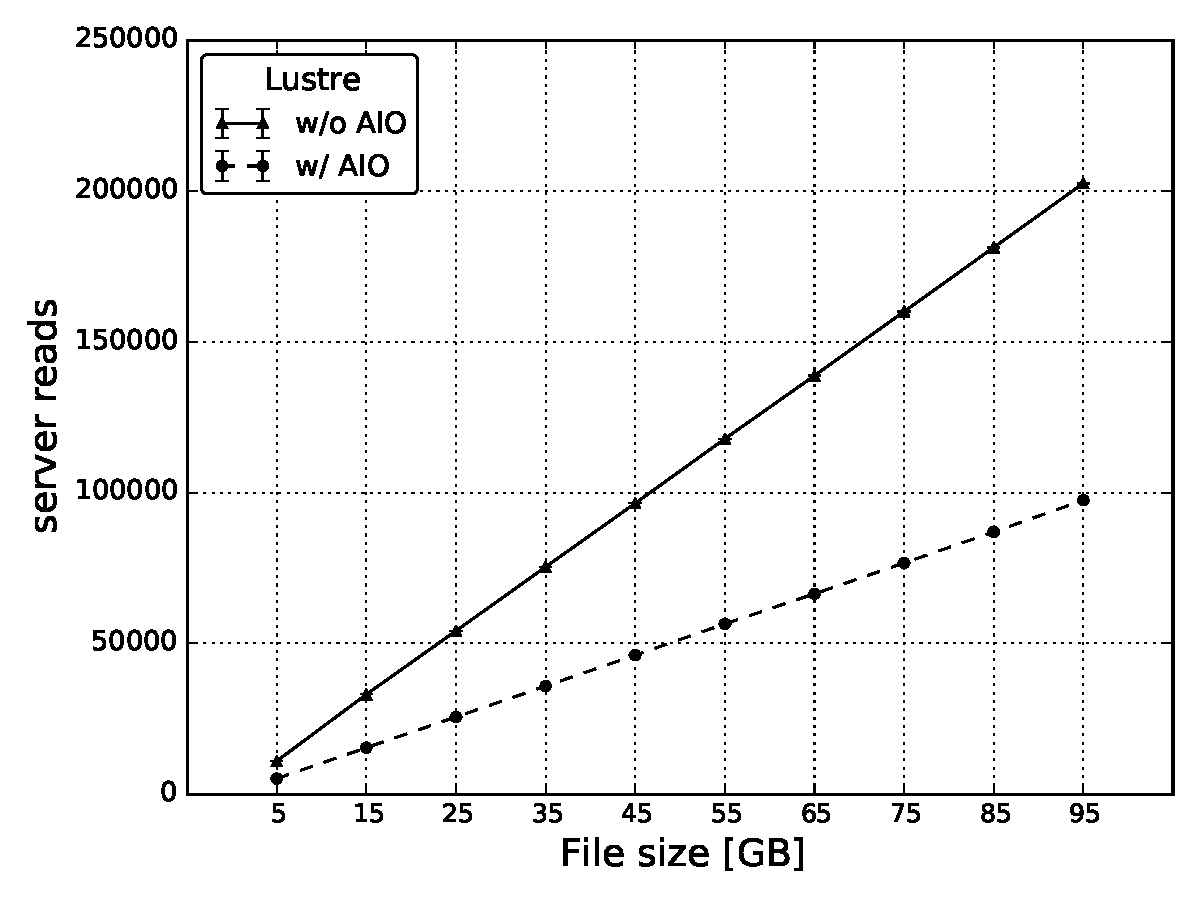
\includegraphics[width=\textwidth]{chapters/chapter2/figures/SC2015/ROOT/separate_plots/test_cluster/Lustre/server_reads}
    \caption{\textit{}}
    \label{figure: lustre_3}
  \end{subfigure}
  \begin{subfigure}[b]{0.32\textwidth}
    \centering
    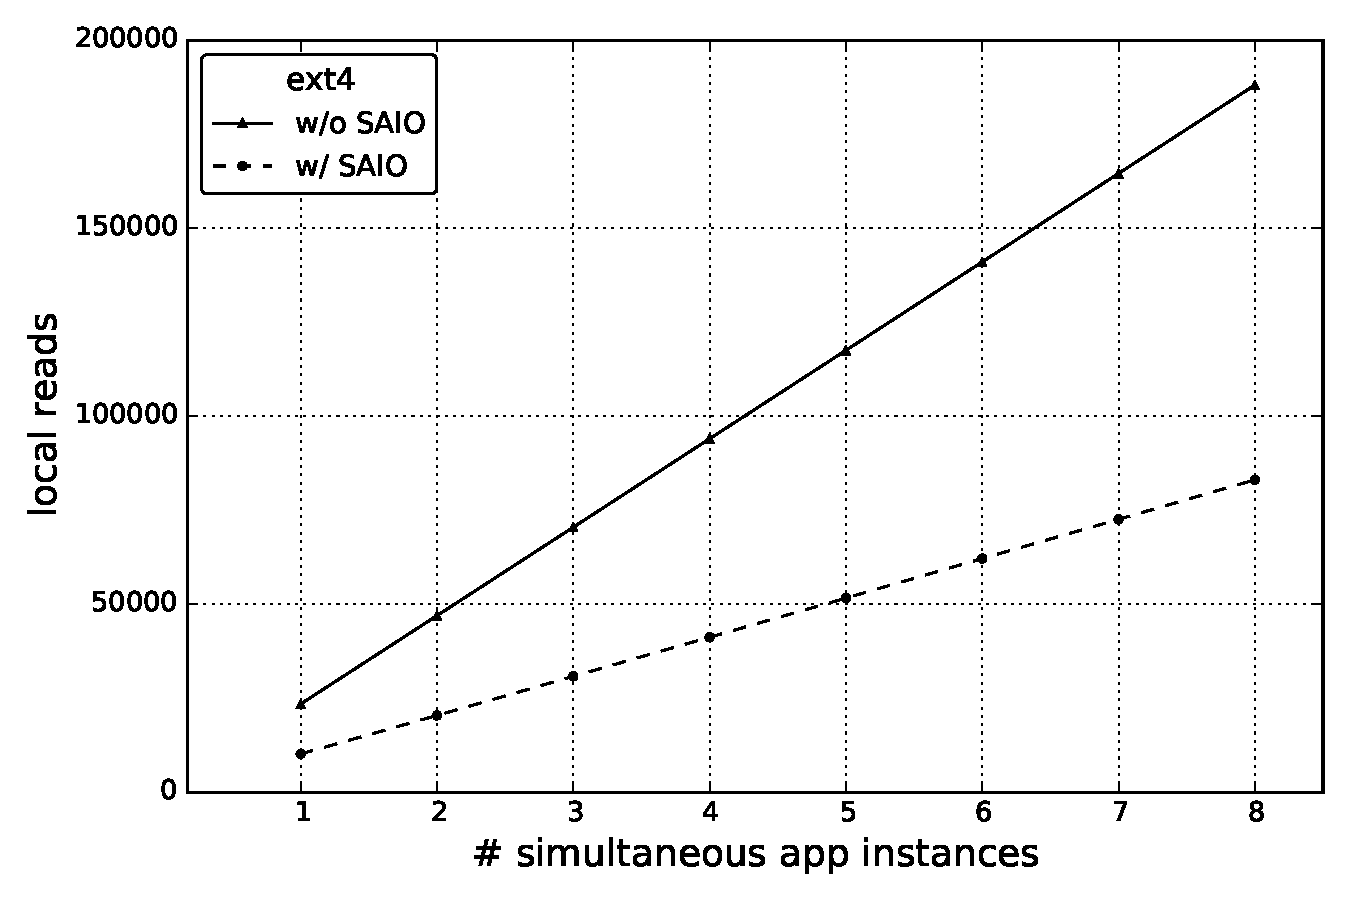
\includegraphics[width=\textwidth]{chapters/chapter2/figures/SC2015/ROOT/cluster/multiple_instances/reads_simult_instance_ext4_test_cluster}
    \caption{\textit{}}
    \label{figure: ext4_4}
  \end{subfigure}
  \begin{subfigure}[b]{0.32\textwidth}
    \centering
    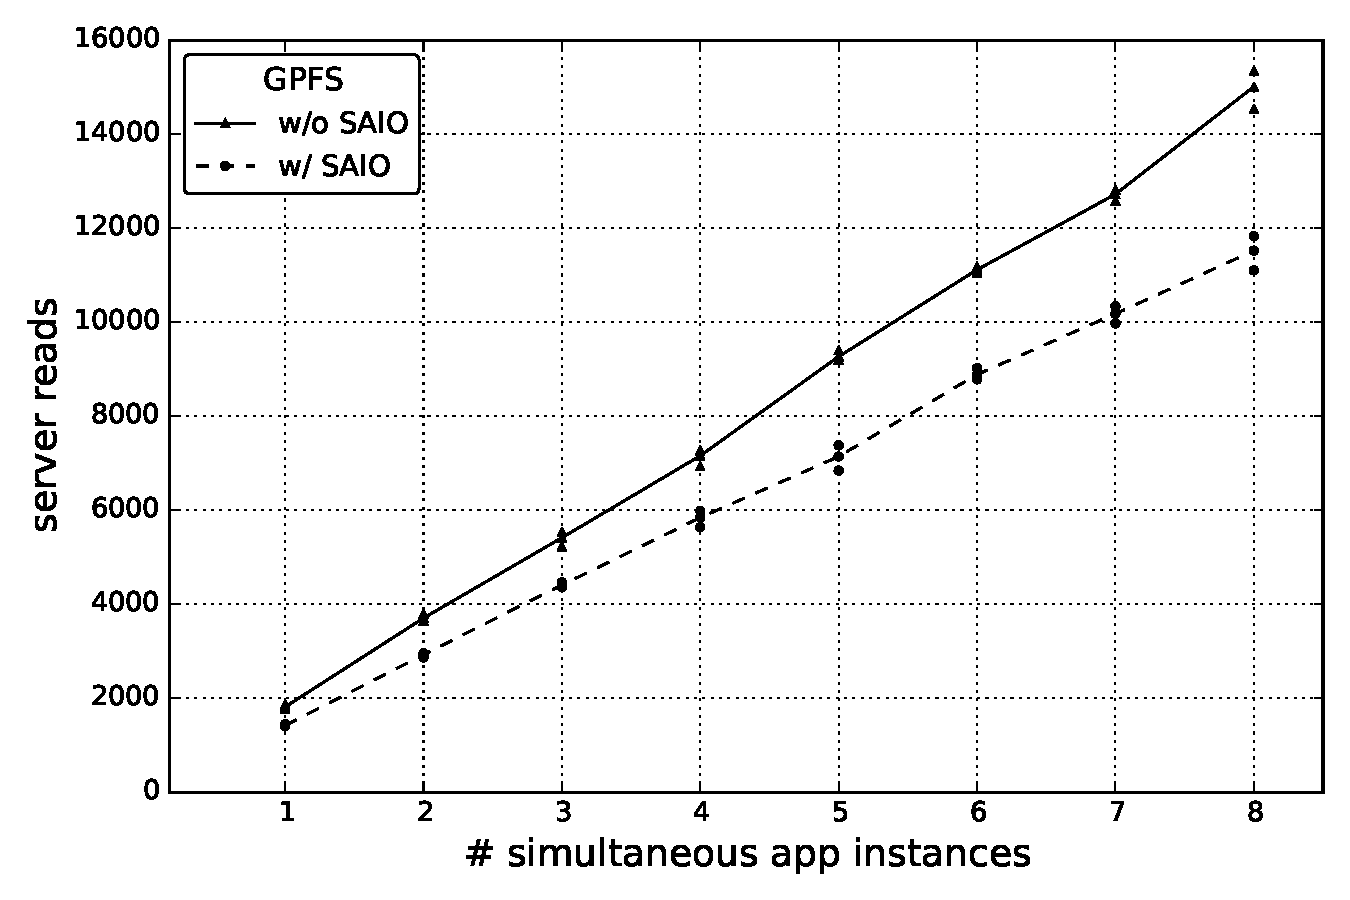
\includegraphics[width=\textwidth]{chapters/chapter2/figures/SC2015/ROOT/cluster/multiple_instances/reads_simult_instance_gpfs_test_cluster}
    \caption{\textit{}}
    \label{figure: gpfs_4}
  \end{subfigure}
  \begin{subfigure}[b]{0.32\textwidth}
    \centering
    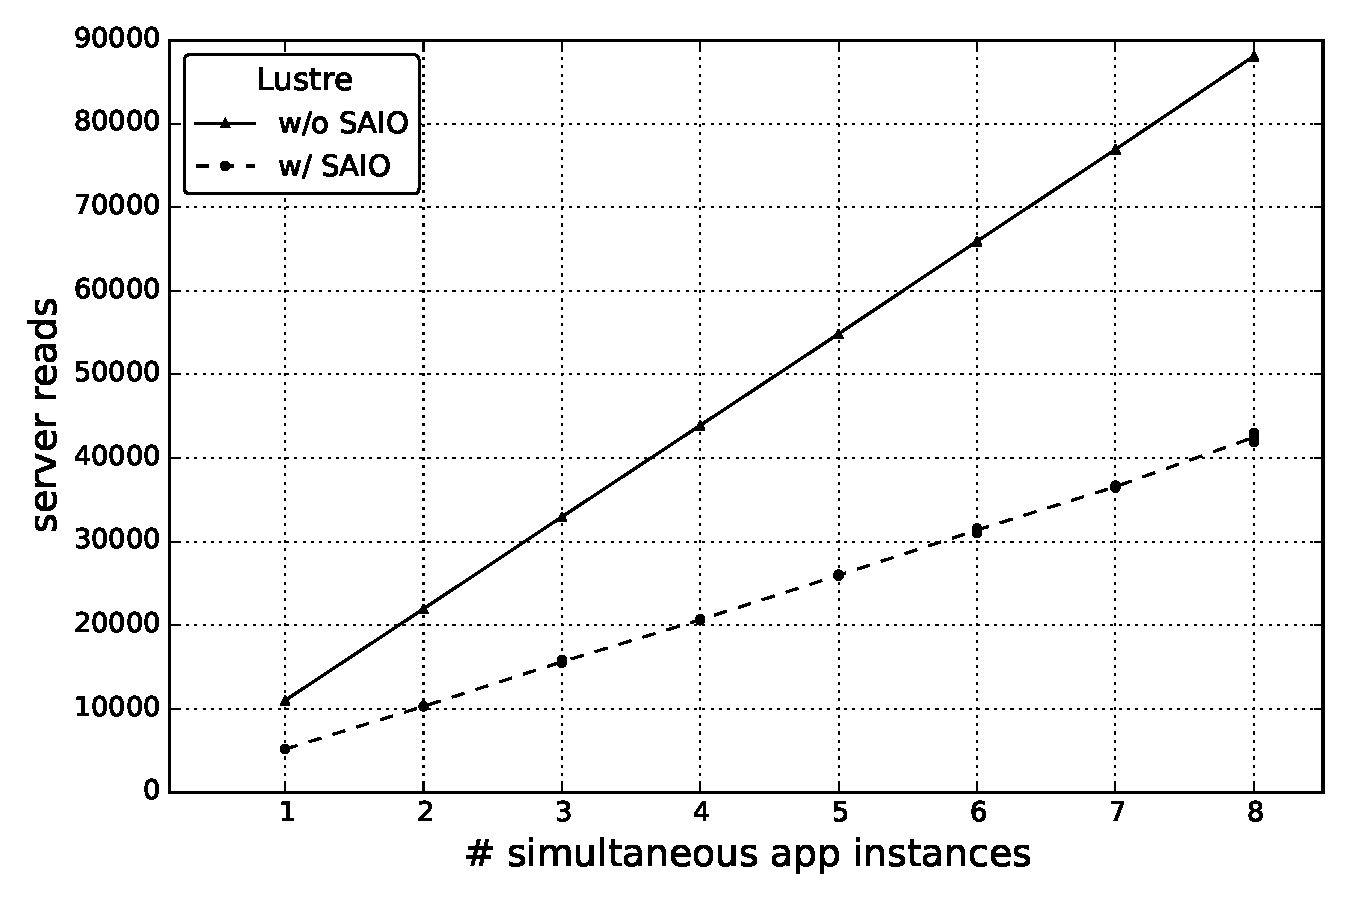
\includegraphics[width=\textwidth]{chapters/chapter2/figures/SC2015/ROOT/cluster/multiple_instances/reads_multiple_simult_procs_Lustre_testcluster}
    \caption{\textit{}}
    \label{figure: lustre_4}
  \end{subfigure}
  \caption{Reads processed by local ext4, GPFS and Lustre I/O servers for various input file sizes (\ref{figure: ext4_3},~\ref{figure: gpfs_3} and~\ref{figure: lustre_3}) and multiple instances of ROOT accessing a file of 5 GB (\ref{figure: ext4_4},~\ref{figure: gpfs_4} and~\ref{figure: lustre_4}).}
  \label{figure: read}
\end{figure*}

As far as Figures~\ref{figure: ext4_2},~\ref{figure: gpfs_2} and~\ref{figure: lustre_2} are concerned, these account for the effect of processes' concurrency on the file system. Before continuing with the discussion we have to make a note here. In our architecture, only one process per file system's client issues (through multiple \textit{Advisor Thread}s) hints on behalf of running applications. This introduces some overhead, since we have to pass the access information from the \textit{Assisted I/O library} to the \textit{Advice Manager}, but has the advantage of better coordinating accesses to the same file from multiple processes. Nevertheless, we found that in the case of GPFS, despite the fact of having multiple \textit{Advisor Thread}s, only one process among the many was receiving a benefit from the prefetching hints. The reason is that GPFS seems to have the restriction of hinting only one file per process. For this reason, we developed another variant of MERCURY in which the AIO library, now renamed \textit{Self Assisted I/O library} (SAIO), internally provides the creation and the handling of multiple \textit{Advisor Thread}s. Looking at the figures generated with the new SAIO library we can assess the effectiveness of the prefetching hints for the three file systems considered. In particular, Lustre provides the best runtime improvements compared to the case in which no hints were used. GPFS shows a more contained improvement since the I/O time is already small compared to Lustre and ext4. Finally, ext4 can really benefit from prefetching hints especially for high process counts. Overall, excluding ext4, when we increase the number of processes the runtime improvements shrink. This is probably due to the saturation of the file system client bandwidth.

\subsection{Read Request Rate}
\label{subsec: reads}
Figure~\ref{figure: ext4_3},~\ref{figure: gpfs_3} and~\ref{figure: lustre_3} report the number of read requests accounted for by the different file systems under study. In the specific, the figures show how the number of reads at the I/O server side for both GPFS and Lustre can be substantially reduced with our approach. This has a significant impact in HPC cluster in which the file system may be accessed by many thousand of processes at the same time. Reducing the number of requests for an application can increase the number of IOPS available for others. This result is also confirmed for multiple instances of the `ROOT' application running concurrently (Figure~\ref{figure: ext4_4},~\ref{figure: gpfs_4} and~\ref{figure: lustre_4}).
